\chapter{Распознавание изображений}
\section{Базовые понятия}
\begin{definition}
Растровое изображение есть функция $$I_{rgb}(x,y): N \times N \to([0,255],[0,255],[0,255])$$ 
\end{definition}
Таким образом каждой точке $(x,y)$ мы сопоставляем тройку $(r,g,b)$. Первый элемент тройки соответствует красной компоненте цвета в растровом изображении, второй -- зеленой и третий -- синей. Далее, для краткости, будем использовать следующую запись:

$$
\begin{array}{l}
I_r(x,y) = I_{rgb}(x,y)_r \text{ -- красная компонента}\\
I_g(x,y) = I_{rgb}(x,y)_g \text{ -- зеленая компонента}\\
I_b(x,y) = I_{rgb}(x,y)_b \text{ -- синяя компонента}\\
\end{array}
$$

\begin{definition}
Определим растровое изображение заданного в оттенках серого как функцию
$$I_{grey}(x,y): N \times N \to[0,255]$$
\end{definition}

\begin{definition}
Введем оператор <<обесцвечивания>> $D$, который обеспечивает переход от цветного изображения $I_{rgb}$ к изображению $I_{grey}$, заданному в оттенках серого:
$$D(I_{rgb}) = I_{grey}$$
\end{definition}

Существует несколько основных способов обесцвечивания изображения:
\begin{enumerate}
 \item Красный канал $D_{red}(I_{rgb}) = I_r$
 \item Зеленый канал $D_{greeb}(I_{rgb}) = I_g$
 \item Синий канал $D_{blue}(I_{rgb}) = I_b$  
 \item Среднее значение (average): $D_{avg}(I_{rgb}) = \frac{I_r + I_g + I_b}{3}$
 \item Лума (luma), учитывает особенности восприятия цвета человеком: $$D_{luma}(I_rgb) = I_r\cdot0.3 + I_g\cdot0.59 + I_b\cdot0.11$$
 		Значения коэффициентов, иногда, могут отличаться от приведенных выше, но их сумма всегда равна 1
 \item Минимум  $D_{min}(I_{rgb}) = min(I_r, I_g, I_b)$
 \item Максимум  $D_{min}(I_{rgb}) = max(I_r, I_g, I_b)$
 \item Обесцвечивание (desaturtaion): $D_{desaturation}(I_{rgb}) = \frac{D_{min}(I_{rgb}) + D_{max}(I_{rgb})}{2}$
\end{enumerate}

\begin{figure}[h]
\centering
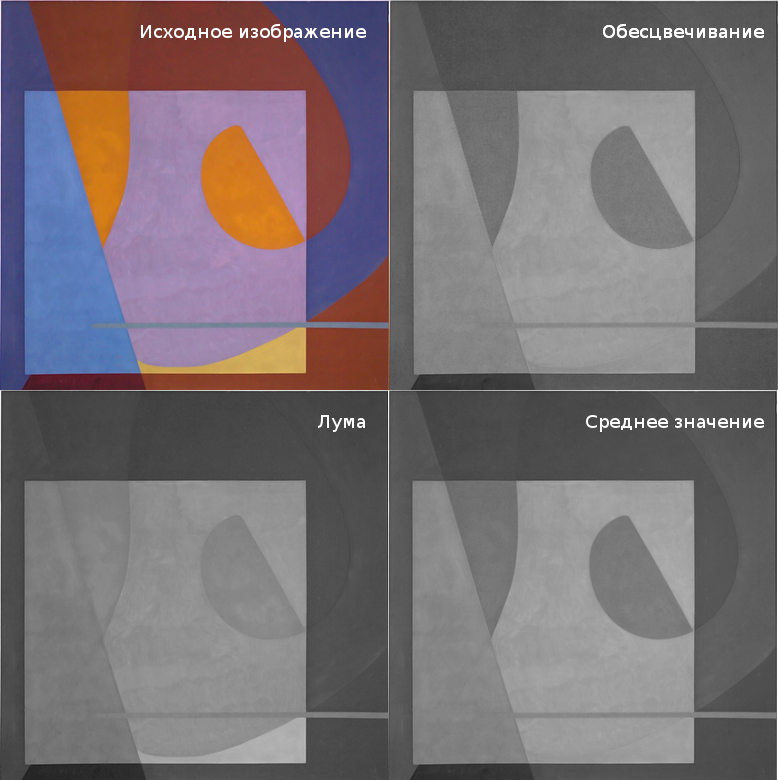
\includegraphics[width=0.75\linewidth,keepaspectratio]{images/th_desaturate}
\caption{Сравнение методов обесцвечивания}
\end{figure}

\begin{remark}
Наилучший результат для средне-статистического изображения (с гистограммой близкой к нормальной) получается при использование 5-го и последнего способов. Под наилучшим результатом понимается сохранение яркости (компоненты value в модели HSV) цветов исходного изображения.
\end{remark}

\begin{definition}
Растровое монохромное изображение есть функция 
$$I_m(x,y): N \times N \to \{0,1\}$$
\end{definition}

Переход от изображения заданного в оттенках серого к монохромному изображению осуществляется через операцию отсечения. Операция отсечения реализуется через оператор отсечения $T$, для некоторого фиксированного $t\in[0,255]$
\begin{definition}
Оператор отсечения $T$ есть:
$$
T(t, I_{grey}) = \left\{ 
\begin{array}{ll}
1 & ,I_{grey} < t \\
0 & ,\text{иначе} 
\end{array}
\right\}
$$
\end{definition}
Таким образом монохромное изображение есть $I_m = T(t, I_{grey})$

\begin{remark}
Значение $t$ определяется опытном путем и зависит от исходного изображения. Для рукописного текста написанного черной ручкой на офисной бумаге берутся значения близкие к 100 (чем меньше значение, тем темнее изображение).
\end{remark}
%TODO последовательность изображений показывающих переход от цветного изображения -> к серому -> к монохромному

\begin{remark}
В данной работе не рассматриваются методы адаптивного отсечения, в силу их медленной производительности излишней в данном контексте точности.
\end{remark}

\begin{definition}
Точки $(x,y)$ для которых верно $I(x,y) = 1$ будем называть заполненными.
\end{definition}

\begin{definition}
Точки $(x,y)$ для которых верно $I(x,y) = 0$ будем называть пустыми.
\end{definition}

Множество заполненных точек образует множество связных областей 
$$\{K_1, K_2 \dots K_n \},$$
таких что:
\begin{enumerate}
\item $\forall(x_1, y_1)\forall(x_2, y_2)(|x_1 - x_2| > 1 \wedge |y_1 - y_2|>1)$, где $(x_1, y_1)\in K_i$, $(x_2, y_2)\in K_j$ и $i\neq j$ 
\item $\forall(x_1, y_1)\exists(x_2, y_2)(|x_1 - x_2| \leq 1 \wedge |y_1 - y_2| \leq 1)$, где $(x_1, y_1),(x_2, y_2)\in K_i$ и $(x_1, y_1)\neq(x_2, y_2)$
\item $|K_i|\geq2$
\end{enumerate}

\begin{definition}
Всякую связную область $K_i$ будем называть контуром
\label{def:contour}
\end{definition}

\begin{definition}
Растровое изображение $I$ содержащие по крайней мере один контур будем называть растровым контурным изображением
\end{definition}

\begin{remark}
Не исключая общности, далее будут рассматриваться только растровые изображения содержащие один контур, а под растровым контурным изображением будет пониматься растровое изображение содержащие только один контур.
\end{remark}

\section{Модель контурного изображение}
В качестве математической модели представления растрового контурного изображения будем использовать четырех-основную алгебраическую систему вида.
\begin{definition}
Контурное изображение (далее, изображение) есть система вида
\begin{equation}
\mathfrak{M} = < A, R, V, M; Sector, Angle, Metric, Relation >
\label{eq:model}
\end{equation}
где
\begin{enumerate}
\item[] $A$ -- множество всевозможных дуг,
\item[] $R$ -- множество связей дуг,
\item[] $V \subset Z$ -- множество допустимых углов (например от 0 до 360 градусов),
\item[] $M \subset Z$ -- множество относительных мер,
\item[] $Sector: A \rightarrow V$ -- задает градусную меру дуги,
\item[] $Metric: A \rightarrow M$ -- функция сопоставляющая каждой дуге ее относительную величину,
\item[] $Angle: R \rightarrow V$ -- задает угол соединения двух дуг
\item[] $Relation: R \rightarrow A \times A$ -- сопоставляет каждой связи дуги, те дуги, которые она соединяет.
\end{enumerate}
\end{definition}

\begin{remark}
Важно отметить, что в этом представлении все множества являются конечными, и, если множества $A$ и $R$ являются фиктивными (чисто техническими элементами) данной модели, и определяются через функции, то множество $V = \{v_0, v_1, ..., v_n\}$ -- есть конечное множество чисел, с максимальным $v_{max}$ и минимальным $v_{min}$ элементами, разбитое шагом $\delta$ на $n+1$ элементов, где 

$$n = \frac{v_{max} - v_{min}}{\delta} $$
$$v_0 = v_{min}$$
$$v_{i} - v_{i-1} = \delta, \forall i=\bar{1,n} $$
$$v_n = v_{max} $$
\end{remark}

\begin{remark}
Как и множество $V$, множество $M$ конечно. Однако выбор верхней границы для $M$ не столь очевиден, так как не исключена возможность того, что разница в размерах между двумя дугами может быть весьма существенна (например в несколько миллионов раз). Однако, в рамках нашей области применения (распознавание символов), когда в качестве <<эталонного наблюдателя>> выступает человеческий глаз, разница что в 1000, что в 1000000 раз почти неразличима, и поэтому ею вполне можно пренебречь, выбрав в качестве максимального значения например 100000 процентов, а в качестве шага одну десятую процента. Таким образом всякая дуга может быть как больше так и меньше любой дуги не более чем в 1000 раз.
\end{remark}

Для наших целей важно всегда работать только с конечными множествами, что достигается рассмотрением конечных множеств $A$, $R$, а также предположением о наличии минимального шага возрастания количественных характеристик дуг и связей дуг.

Таким образом контурное изображение будет представляет собой систему дуг и связей дуг. Где всякая дуга определяется через ее градусную меру и через относительную (в данном контуре) длину дуги. А всякая связь определяется через угол связи и пару дуг которые она связывает.

\section{Преобразование растрового изображения}
Переход от растрового контурного изображения к изображению состоит из двух этапов. Первый этап — волновая скелетизация. С помощью скелетезации на основе растрового изображение строится граф (скелет), который визуально адекватно соответствует исходному изображению.

Пусть $I$ -- растровое контурное изображение и $K$ -- есть его контур.

\begin{definition}
Точку $q(x_1, y_1)$ будем называть соседом точки $p(x, y)$ если $|x-x_1| \le 1$ и $|y-y_1| \le 1$ и $p\neq q$.
Введем отношение соседства $N(p,q)$, которое истинно если $p$ сосед $q$.
\end{definition}

Очевидно что точка $p$ не может иметь более 8 соседей. Обозначим через $N_K^p$ множество всех соседей точки $p(x,y)$ лежащих контуре~$K$:
$$N_K^p = \{q | q\in K \wedge N(p,q)\}$$
Согласно определению контура (\ref{def:contour}) очевидно, что $K$ не имеет изолированных точек т.е.
$$\forall p \exists q: N(p,q)$$
$$p,q\in K$$

\begin{remark}
Скелетом $I$ будем называть граф $G(V,E)$, «интуитивно адекватно отражающий» исходное изображение.
\end{remark}

\begin{definition}
Волной $w$ будем называть конечное множество точек $\{p_j\}$.
\end{definition}

\begin{definition}
Множество волн $\{w_1,w_2,...,w_n\}$ будем называть подволнами волны $w$ если:
$$\bigcup\limits_{i=1,n}{w_i} = w$$
$$w_i\cap w_j = \emptyset,\; i,j = \overline{1,n},\; i\neq j;$$
и для любых двух точек $p\in w_i,\: g\in w_j$, где $i\neq j$ верно $\neg N(p,g)$.
\end{definition}

Введем функцию вычисляющую центр масс точек волны 
$$g(w)=\dfrac{\sum\limits_{p\in w} p}{\lvert w\rvert}$$

\subsection{Волновая скелетизация}
Опишем алгоритм построения скелета растрового контурного изображения.

\begin{figure}[h]
\centering
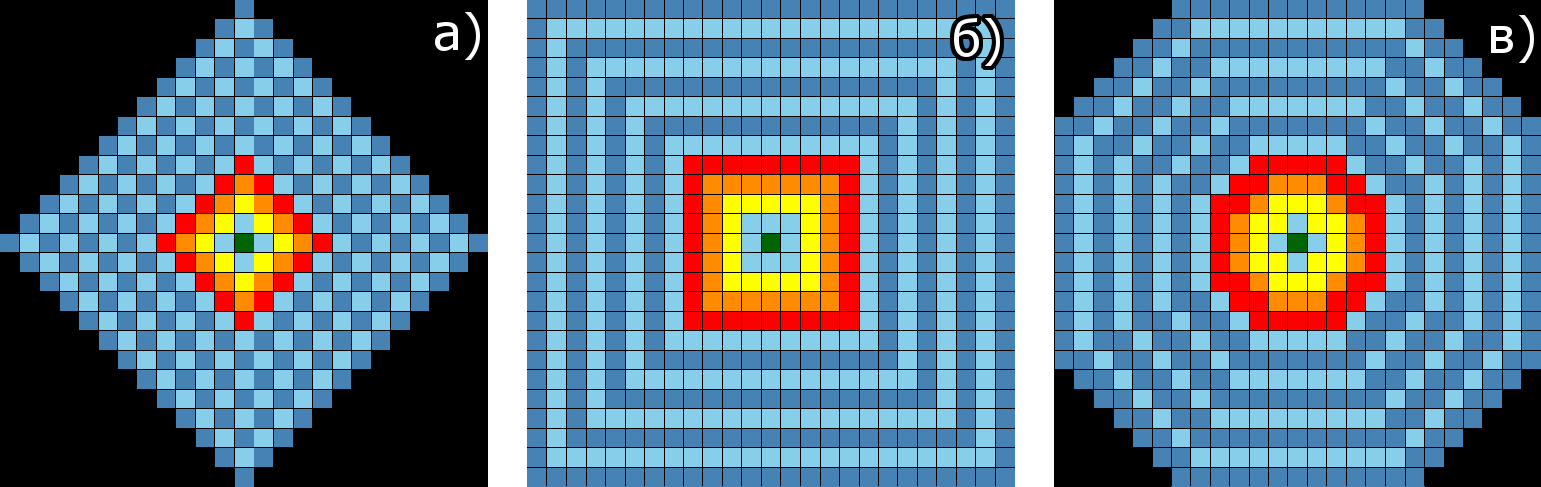
\includegraphics[width=\linewidth,keepaspectratio]{images/th_wave}
\caption{Распространение волны: а)--ромбовидная, б)--квадратная, в)-сферическая }
\end{figure}

%\begin{alg}
Зададим начальные условия. В качестве начальной волны подойдет любая точка из~$F$. 
Имеем следующую начальную конфигурацию:\\
${{w_0}^0} = \{p\}, p\in K$ -- начальная волна,\\
$W_0 = \{{w_0}^0\}$  -- множество волн,\\
$F_0 = K$ -- состояние заполненной области,\\
$G_0(V_0,E_0), V_0=\{p\}, E_0=\emptyset$ - начальное состояние скелета.\\

Определим $n$-ый шаг итерации следующим образом.
Для всякой $i$-ой волны ${w_i}^{k_i-1}$ из $W_{n-1}$ ($k_i$ - соответствует $k_i$-ой итерации $w_i$):
\begin{equation}
{w_i}^{k_i} = \bigcup_{p\in{w_i}^{k_i-1}}N_{F_{n-1}}^p\setminus\bigcup_{j<i}{w_j}^{k_j-1}
\label{skeleton1}
\end{equation}
Если $u_1,\ldots ,u_m$ есть подволны волны ${w_i}^{k_i}$, тогда
$$W^i_n=\{w_{l+1},\ldots ,w_{l+m}\}$$
где
$$w_{l+j}=u_j, j=\overline{1,m}$$
$$l = |W_{n-1}|+\sum\limits_{j<i}|W^j_n|.$$
Ребра в графе образуют вектора, связывающие центры масс полученных подволн с центром массы ${w_i}^{k_i-1}$
$$E^i_n=\{(v_{i}^{k_{i-1}}, v_{l+j}^{k_i})\}, j=\overline{1,m}$$
$$V^i_n=\{v_{l+j}^{k_i}\}, j=\overline{1,m}$$
$$v_i^j = g(w_i^j)$$
Если же волна $w_i^{k_i}$ не имеет разрывов и $w_i^{k_i}\neq\emptyset$, то
$$W^i_n=\{{w_i}^{k_i}\}$$
$$E^i_n=\{(v_{i}^{k_{i-1}}, v_{i}^{k_{i}})\}$$
$$V^i_n=\{v_{i}^{k_{i}}\}$$
Если $w_i^{k_i}=\emptyset$
$$W^i_n=\emptyset,E^i_n=\emptyset,V^i_n=\emptyset$$
Таким образом, при $s_n = |W_{n-1}|$:
$$W_{n} = \{W^i_n\}, i=\overline{1,s_n}$$
$$V_n = V_{n-1}\bigcup_i V^i_n, i=\overline{1,s_n}$$
$$E_n = E_{n-1}\bigcup_i{E^i_n}, i=\overline{1,s_n}$$
$$F_{n} = F_{n-1}\setminus P_{n-1},$$ 
$$P_{n-1} = \{p : p\in w, w \in W_{n-1}\}$$
Если $|F_{n}|=0$ то алгоритм прекращает цикл итераций, а граф
$$G = (V_n, E_n)$$
является скелетом исходного изображения $f$.\\

\begin{state} 
Алгоритм волновая скелетизация остановится на всяком контуре мощности $m$
\end{state}

\begin{proof}
Пусть $m=1$, тогда 
$$|F_1|=|F_0\setminus\{p:p\in w, w\in W_0\}| = |\{p\}\setminus\{p:p\in w_0\}|=|\{p\}\setminus\{p\}|=\emptyset$$
следовательно алгоритм прекращает свою работу а граф $G=(V_1,E_1)=(\{p\},\emptyset)$ является скелетом изображения.\\Пусть $m>2$. От противного: допустим, что существует такое $l$ что для всякого $k<l,|F_{k}| < |F_{k-1}|$ и $|F_{l}|=|F_{l-1}|$, тогда $P_{n-1}=\emptyset$, отсюда следует, что $\{p : p\in w, w \in W_{n-1}\}=\emptyset$, а это возможно только в двух случаях:\\
\begin{enumerate}
\item если $W_{n-1}$ пусто, тогда, в силу~\ref{skeleton1} и в силу отсутствия изолированных точек, $F_{n-2}=\emptyset$, получаем противоречие с условием остановки.\\
\item если $\forall w\in W:|w|=0$, тогда, опять же в силу~\ref{skeleton1} и в силу отсутствия изолированных точек, получаем что $F_{n-2}=\emptyset$, снова получаем противоречие с условием остановки.\\
\end{enumerate}
Следовательно такого $l$ не существует, и алгоритм сходится для всякой непустой заполненной области без изолированных точек.
\end{proof}
\begin{figure}[h]
\centering
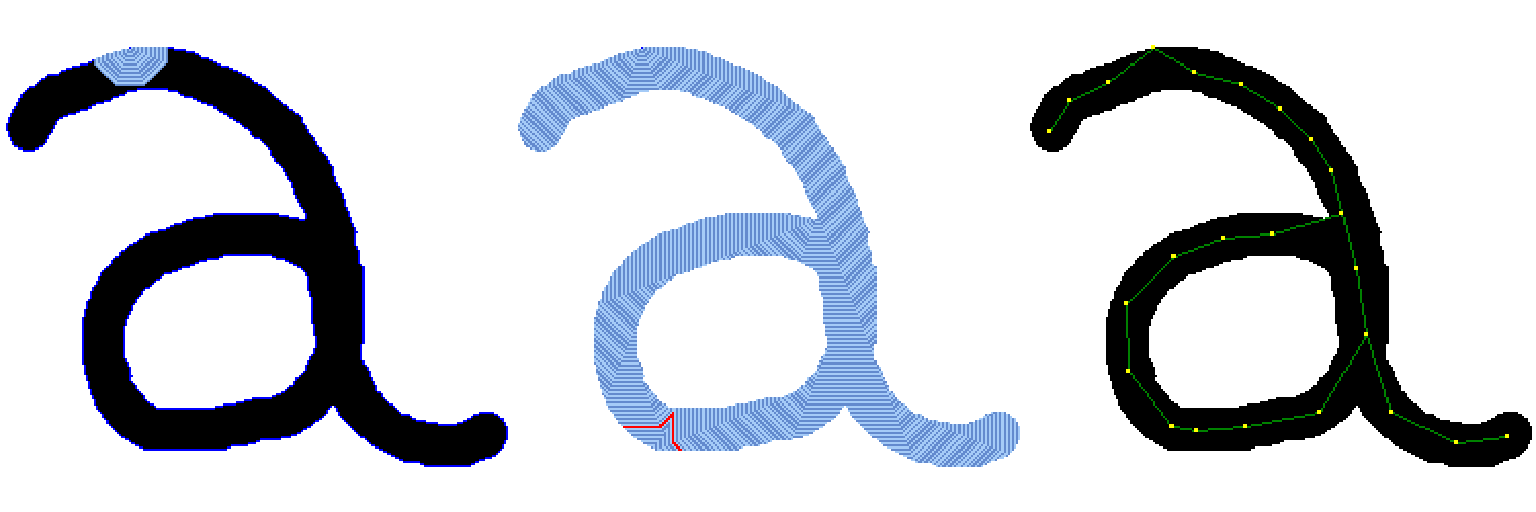
\includegraphics[width=\linewidth,keepaspectratio]{images/th_wave_graph}
\caption{Распространение волны по области, на последнем изображении представлен полученный граф}
\end{figure}

\subsection{Построение модели  $\mathfrak{M}$ для графа $G$}
Рассмотрим схему разбиения графа особыми точками

\begin{figure}[h]
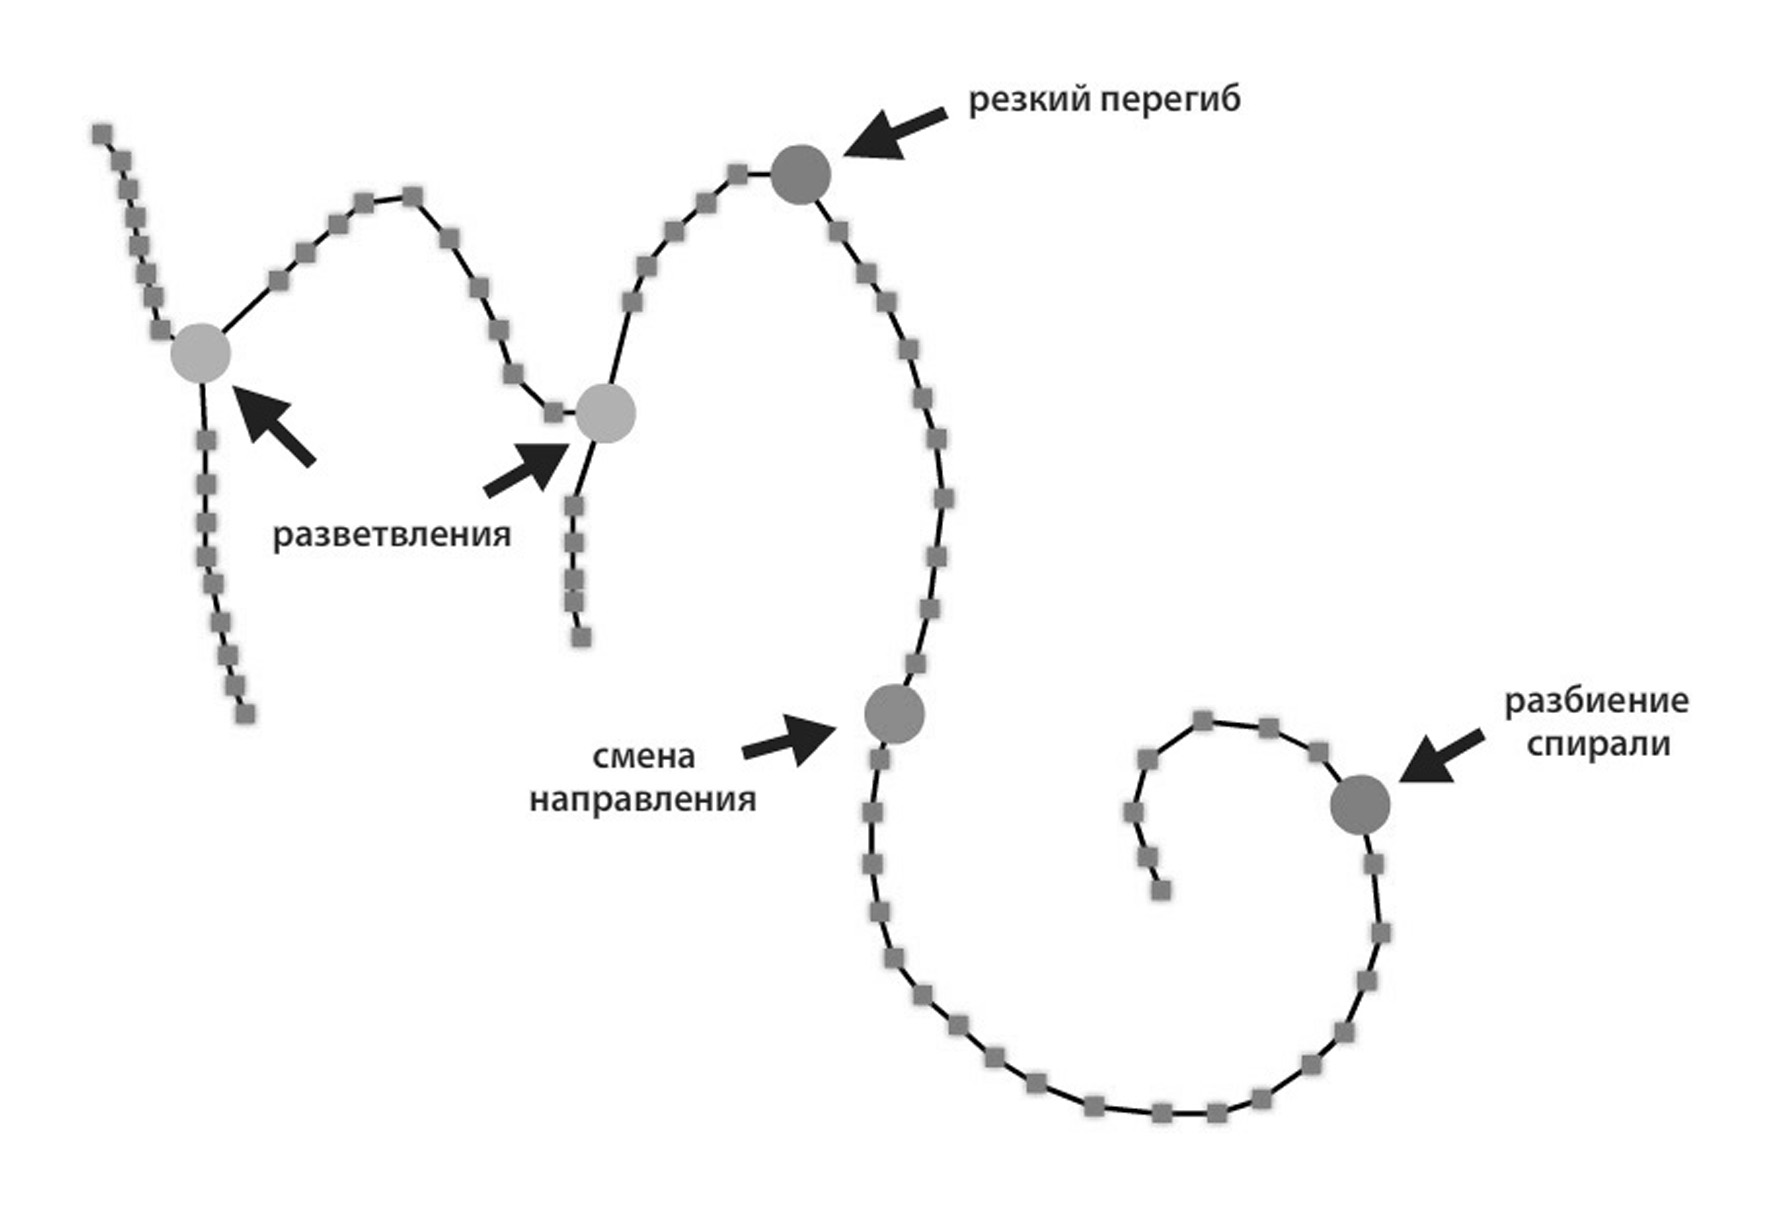
\includegraphics[width=\linewidth,keepaspectratio]{images/th_peregib}
\caption{Схема разбиения графа «особыми» точками}
\end{figure}

\begin{enumerate}
\item Для каждого простого пути выполняется:
	\begin{enumerate}
		\item Разбиение пути по точкам смены направления обхода
		\item Для каждого разбиения выполнятся
		\begin{enumerate}
			\item Разбиение спиралей. Чтобы определить закручен ли путь по спирали, надо проверить пересекает ли хорда путь. Если пересечение есть, то необходимо разбить путь точками пересечения
			\item Для каждого разбиения выполняется:
			\begin{enumerate}
				\item Разбиение по точкам перегиба. Точками перегиба считаются образующие две дуги отклонившиеся от угла идеального соединения. Угол $\gamma$ идеального соединения двух дуг градусной меры $\alpha$ и $\beta$: $$\gamma=2\pi-(\alpha+\beta)$$
			\end{enumerate}
		\end{enumerate}		
	\end{enumerate}	
\item Результатом п.1 является множество подпутей, каждый из которых переводится в дугу. Градусная мера дуги вычисляется с использование формулы Гюйгенса. Определив наиболее удаленную точку пути от хорды стягивающей путь, и вычислив её положение относительно хорды направленной от начала к концу пути, мы определяем направление обхода. Если точка слева, то обход ведется по часовой стрелке, если точка справа — обход ведется против часовой стрелки, если же точка лежит на прямой, то верны оба утверждения.
\item Расчет связей дуг. Связь между двумя дугами существует, если пути образующие дуги имели общие вершины. Угол соединения между дугами рассчитывается, как угол между стягивающими их хордами
\end{enumerate}

\begin{remark}
Стоит отметить что разбиение на дуги, как правило, выполняется на интерполированном графе в котором часть узлов удаленно в силу их избыточности. 
\end{remark}

\begin{remark}
Хотя разбиение и может быть использовано как есть, на практике полезнее добавлять возможность вариации параметров, например, допускать возможность некоторого отклонения от угла идеального соединения или для точек смены направления расширять область проверки на смену направления обхода.
\end{remark}

Пусть $\{P_1, P_2, \dots, P_m\}$ -- множество простых цепей графа $G=(V,E)$ таких что:
\begin{enumerate}
\item $P_i = v^i_1, v^i_2, \dots v^i_{n_i}$
\item $\forall v\in P_i \forall u \in P_j(v\neq u)$, где $i\neq j$
\item $d(v^i_1)\neq 2$ и $d(v^i_{n_i})\neq 2$
\item $\forall j\notin\{1, n_i\}\left[d(v^i_j) = 2\right]$
\item $\bigcup_i P_i = V$
\end{enumerate}
%TODO добавить частный случай о графе образованного одним циклом (буква О)

\begin{definition}
Пусть $r(p,v)$ -- есть растояние от точки $p$ до вектора $v$ со знаком
\end{definition}


\begin{definition}
Будем говорить что в узле $v_i$ меняется направление обхода простого  
$$\{v_1,...,v_{i-1},v_i,v_{i+1},...,v_n\}$$
в окрестности $\epsilon\in \{2, 3, ...\}$, если
$$
Sign(\sum\limits_{j=i-\epsilon}{r(v_j,h)}) \neq Sign(\sum\limits_{j=i+\epsilon}{r(v_j,h)})
$$
где $h = (v_{i-\epsilon}, v_{i+\epsilon})$

Если соотношение выполняется для $\epsilon=2$ будем просто говорить, что в точке $v_i$ меняется направление обхода.
\end{definition}

Пусть множество точек  $\{ v_{j^i_{1}}, \dots v_{j^i_{k_i}} \}$ множество точек смены направления обхода цепи $P_i$.
Определим множество индексов задающих разбиение пути $P_i = v_1, \dots v_n$ по направлению обхода
$$
I^{dev}_{P_i} = \{ j^i_{1}, \dots j^i_{k_i} \} \cup \{1, n\}
$$
$$
j^i_{k} < j^i_{k+1}
$$
Тогда следующие семейство множеств узлов определяют разбиение пути $P_i$ на подпути:
$$
S^{dev}_{P_i} = \bigcup_{l \in I^{dev}_{P_i}}
	\{
		\{ v_t\;|\;t\in \{j\;|\;i_l\leq j\leq i_{l+1}\}\}
	\}
$$
Каждому множеству узлов можно однозначно сопоставить подпуть $P_i$

\begin{definition}
Определим множество индексов узлов задающие разбиение подпути $P = v_1, \dots v_n$ закрученного в спираль следующим образом
$$I^{spir}_P = \left\{ \min_{|r(h, v_i)|}(i, i+1)\;|\;Sign(r(h,v_i)) \neq Sign(r(h,v_{i+1})) \wedge i=1,n-1 \right\}
$$
$$
h = (v_1, v_n)
$$
%TODO картинка цепи закрученной в спираль
\end{definition}

\begin{definition}
Определим множество индексов узлов задающие разбиение подпути $P = v_1, \dots v_n$ по резкости угла перегиба.

\end{definition}

\begin{definition}
Разбиением пути $P$ на характеристические подпути будем считать разбиение определенное следующим образом:

$$
S_{P_i} =
 	\bigcup_{ j\in I^{spir}_P,\;P\in S^{dev}_{P_i}} 
 	\left\{
 	 	\left\{
 	 		 v_t\;|\;t\in\{j\;|\;i_l\leq j\leq i_{l+1} \} 
 	 	\right\}	 
 	 \right\}
$$
\end{definition}

\begin{definition}
Пусть $P = v_1, \dots v_n$ простой путь тогда:
\begin{enumerate}
\item $f_{begin}(P) = v_1$ -- начало пути
\item $f_{end}(P) = v_n$ -- конец пути
\item $h_P = v_n - v_1$ -- вектор хорды стягивающей путь
\end{enumerate}
\end{definition}

\begin{definition}
Пусть задано разбиение графа $G=(V,E)$ на характеристические подпути $S=\{P_1, \dots P_m\}$, где $P_i=v^i_1, \dots v^i_{n_i}$, будем говорить что алгебраическая система
$$\mathfrak{M} = < A, R, V, M; Sector, Angle, Metric, Relation >$$
соответствует графу $G$ если выполняются следующие условия:
\begin{enumerate}
\item $Sector(a_i) = 2l + \frac{1}{3}(2l - L)$, где $l=|v^i_1-v^i_m|$, $i_m = \frac{n_i}{2}$,  а $L=|h_{P_i}|$
\item $Metric(a_i) = \frac{a_i}{a_1}$
\item $Relation(r_{ij}) = (a_i, a_j)$, где $i\neq j$ и неопределенно в противном случае
\item $Angle(r_{ij})=
	\left\{		
	\begin{array}{ll}
	\hat{(-h_{P_i}, -h_{P_j}}) & f_{begin}(P_i) = f_{end}(P_j) \\
	\hat{(-h_{P_i}, h_{P_j}}) & f_{begin}(P_i) = f_{begin}(P_j) \\
	\hat{(h_{P_i}, h_{P_j}}) & f_{end}(P_i) = f_{begin}(P_j) \\
	\hat{(h_{P_i}, -h_{P_j}}) & f_{end}(P_i) = f_{end}(P_j) \\	
	\text{неопределенно}, & \text{если } r_{ij} \text{ -- неопределенно}
	\end{array}
	\right\}	$	
\end{enumerate}
\end{definition}

\section{Постановка задачи анализа плоских контурных изображений }
Пусть изображение есть модель следующего вида:
\begin{equation}
\mathfrak{M} = < A, R, V; Sector, Angle, Relation >
\label{vipeq1}
\end{equation}

\begin{equation}
M_{ini} = <A_1,...,A_s;f_1,...,f_n;p_1,...,p_k>
\label{vipeq2}
\end{equation}
где $A_i$ -- основные множества, $f_i$ -- операции (функции) на основных множествах, $p_i$ -- предикаты (отношения) на основных множествах, в конечную (финальную) $M_{fin}$, удовлетворяющую ограничениям $R_1,R_2,...,R_m$.

Если искать аналоги, то последовательность таких преобразований можно считать допустимым (без оптимизации значений целевого функционала) управлением для задачи динамического программирования~\cite{9}, где $R_1,R_2,...,R_m$ фазовые ограничения.

При программной реализации многоосновная а.с.~\ref{vipeq2} становится реляционной БД, поиск последовательности преобразований для построения финальной а.с., удовлетворяющей ограничениям – комбинаторной задачей высокой сложности.

Для рассматриваемой здесь предметной области (анализ изображений) общая схема решения пока не может быть применена в полном объеме из-за начального этапа исследований (с точки зрения логико-эвристических методов) и отсутствия конкретных постановок прикладных задач (ближайшие планы применения логико-эвристических методов обсуждаются в заключении).

Поэтому ограничимся исследованием сложности проверки выполнимости ограничений $R_1,R_2,...,R_m$ на математических моделях вида~\ref{vipeq1} с позиции обеспечения независимости скорости проверки от числа ограничений.

Проверка выполнимости ограничений сводится к проверке вложимости обобщенных изображений (образцов) в анализируемое изображение~\ref{vipeq1}. 

Уточним формализацию описания плоских контурных изображений для данного варианта проверки выполнимости ограничений.

Составляющими элементами образцов и анализируемого изображения будут также дуги и связи дуг. Численными характеристиками которых будут количество минимальных шагов возрастания для дуги (связи дуг) -- градусные меры дуг, имеющие минимальное и максимальное значения.

Таким образом, одноместная функция $Sector: Arc \rightarrow V$ преобразуется в одноместную же функцию $Sector: Arc \rightarrow V \times V$, соответственно, одноместная функция $Angle: Rel \rightarrow V$ преобразуется в одноместную же функцию $Angle: Rel \rightarrow V \times V$.

\begin{remark}
В принципиальном плане ввод минимальных и максимальных значений ничего нового не дает (от минимального до максимального всего конечное множество значений), но позволяет более компактно задавать искомые образцы. Для упрощения технических деталей будем считать, что для анализируемых изображений функции $Sector$ и $Angle$ имеют одинаковое минимальное и максимальное значение
\end{remark}

Пусть многоосновные а.с.
\begin{equation}
	\begin{array}{c}
	R_1=<Arc_1, Rel_1, V; Sector, Angle, R> \\
	R_2=<Arc_2, Rel_2, V; Sector, Angle, R> \\
	\dots\\
	R_m=<Arc_m, Rel_m, V; Sector, Angle, R> \\
	\end{array}
	\label{vipeq3}
\end{equation}
задают искомые образцы в анализируемом изображении~\ref{vipeq1}.

Анализ изображения~\ref{vipeq1} состоит в поиске всех изоморфных вложений ${ \mu_{i,j} }$ многоосновных а.с. $R_1,R_2,...,R_m$ в многоосновную а.с. $M$~\ref{vipeq1}, т.е. изоморфное вложение $\mu_{i,j} : R_i \rightarrow M$ состоит из инъективных отображений
\begin{equation}
\mu_{i,j} : Arc_i \rightarrow Arc; \mu_{i,j} : Rel_i \rightarrow Rel
\label{vipeq4}
\end{equation}

такие, что:

\begin{enumerate}
\item[а)] если $\mu_{i,j}(Ar) = Arr$,где $Ar \in Arc_i$, $Arr \in Arc$, $Sector(Ar) = (v_1, v_2)$, $Sector(Arr) = (v_3, v_4)$, то $v_1 \le v_3 \le v_4 \le v_2$;
\item[б)] если $\mu_{i,j}(Re) = Ree$, где $Re \in Rel_i$, $Ree \in Rel$, $Angle(Re) = (v_1, v_2)$, $Angle(Ree) = (v_3, v_4)$, то $v_1 \le v_3 \le v_4 \le v_2$;
\item[в)] если $R(Re, Ar_1, Ar_2)$, где $Re \in Rel_i$, $Ar_1 \in Arc_i$, $Ar_2 \in Arc_i$, то $R(\mu_{i,j}(Re), \mu_{i,j}(Ar_1), \mu_{i,j}(Ar_2))$.
\end{enumerate}

\section{Оценка сложности анализа изображений}
Для облегчения понимания идеи доказательства основного результата, рассмотрим доказательство теоремы. Основой его является представление декартова произведения конечных множеств.

$$A_1 \times A_2 \times \ldots \times A_n$$
в древовидной форме Tree~\cite{1}.

Определим более точно конечные множества 
\begin{equation}
\begin{array}{c}
A_1 = \{a_{1,1}, a_{1,2}, ..., a_{1,m_1}\}; \\
A_2 = \{ a_{2,1}, a_{2,2}, ..., a_{2,m_2}\}; \\
\dots \\
A_n = \{ a_{n,1}, a_{n,2}, ..., a_{n,m_n}\}; \\
\end{array}
\end{equation}

%\begin{figure*}[b]
%\includegraphics[width=\linewidth,keepaspectratio]{MartyanovKatashevtsev_tbl1}
%\caption{Схема 1. Дерево Tree}
%\end{figure*}

Понятно, что таблица~1 является универсумом для любых таблиц реляционной БД с доменами $A_1, A_2,\ldots,A_n$. Т.е представление отношения $H$ в таблице состоит в пометке вершин $n$-го этажа, если путь от корня дерева до этой вершины $n$-го этажа, дает кортеж из отношения $H$.

Проверка принадлежности кортежа $(a_1,a_2, ..., a_n)$, где $a_1 \in A_1$, $a_2 \in A_2, ..., a_n \in A_n$, отношению $H$ производится за $n$ шагов в таблице~1(этот процесс в дальнейшем будем называть интерпретацией кортежа $(a_1,a_2, ..., a_n)$ на дереве $Tree$). Действительно, $a_1$ позиционируется на 1-ом этаже за 1 шаг, $a_2$ позиционируется на 2-ом этаже за 1 шаг и так далее, $a_n$ позиционируется на $n$-ом этаже за 1 шаг, где и определяется принадлежность кортежа $(a_1,a_2, ..., a_n)$ отношению $H$.

Таким образом, проверка осуществляется за $n$ шагов. Для доказательства теоремы $А$ достаточно пометить вершины $n$-го этажа на принадлежность отношениям $H_1, H_2, ..., H_k$ . Тогда в результате интерпретации кортежа $(a_1,a_2, ..., a_n)$ за $n$ шагов на дереве $Tree$ получим вершину $n$-го этажа пометки которой покажут принадлежность (или не принадлежность) отношениям $H_1, H_2, ..., H_k$.

Оценка $O(n+k)$, а не $O(n)$, получается из-за необходимости пройти по списку отметок $n$-го этажа, что и дает добавку $O(k)$.

\begin{remark}
Результат теоремы~\ref{vipth3} типичный, так называемый обмен памяти на эффективность~\cite{5}.
Конечно, задание декартово произведения деревом увеличивает необходимый объем памяти, но скорость выполнения операций предельно ускоряется. Следует отметить также, что на практике универсум (схема 1) не строится, а строится только его часть, состоящая из кортежей отношений $H_1, H_2, ..., H_k$. Вообще говоря, это замедляет скорость интерпретации, но незначительно не более, чем на $ln(m)$, где $m = max\{ m_1, m_2, …, m_n\}$ 
(это связанно с необходимостью перебора узлов "частичного" дерева, что, в силу упорядоченности, можно реализовать с помощью бинарного поиска).
\end{remark}

Прежде, чем перейти к изложению основного результата, определим универсум для изображений, имеющих не более $n$ дуг, и $k$ вариантов дуг и связей дуг, т.е. множество $V$ имеет $k$ элементов, а минимальный сектор дуги или угол пересечения дуг равен $(360/k)$ градусов.

Пусть $Arc_1, Arc_2, ..., Arc_n$ – множества дуг всех характеристик (образцов), т.е.
\begin{equation}
\begin{array}{c}
Arc_1 = \{ar_{1,1}, ar_{1,2}, ..., ar_{1,m_1}\}; \\
Arc_2 = \{ ar_{2,1}, ar_{2,2}, ..., ar_{2,m_2}\}; \\
\dots \\
Arc_n = \{ ar_{n,1}, ar_{n,2}, ..., ar_{n,m_n}\}; \\
\end{array}
\end{equation}

Далее пусть $Rel_1, Rel_2, ..., Rel_{n-1}$ – множества связей дуг всех характеристик, т.е. 
\begin{equation}
\begin{array}{c}
Rel_1 = \{re_{1,1}, re_{1,2}, ..., re_{1,k_1}\}; \\
Rel_2 = \{ re_{2,1}, re_{2,2}, ..., re_{2,k_2}\}; \\
\dots \\
Rel_{n-1} = \{ re_{{n-1},1}, re_{{n-1},2}, ..., re_{{n-1},k_{n-1}}\}; \\
\\
Angle(re_{i,j})=(j,j)
\end{array}
\end{equation}

Дерево $TreeImage$ (универсум (схема 2) для всех изображений, имеющих не более $n$ дуг, и $k$ вариантов дуг и связей дуг) строится по аналогии с деревом $Tree$ для декартова произведения
$$Arc_1 \times Rel_1 \times Arc_2 \times Rel_2 \times ... \times Rel_{n-1} \times Arc_n $$

%\begin{figure}[b]
%\includegraphics[width=\linewidth,keepaspectratio]{MartyanovKatashevtsev_tbl2}
%\caption{Схема 2. Дерево TreeImage}
%\end{figure}

Соглашения по представлению элементов схемы~2 следующие:
\begin{enumerate}
\item для элемента $\alpha_{\mu,\chi}^\theta$ - число $\theta$ является позицией на этаже схемы (номер клетки в строке); $\alpha_{\mu,\chi}^\theta$ является $\chi$-ым элементом из множества $Arc_{\mu}$ или $Rel_{\mu}$;
\item числа $m_i$, где $i$ - номер этажа, равны $k^i - k$; число $t = k^{2n-1}-k$, отметим, что данные числа имеют чисто технический характер и уменьшают громоздкость выражений, стоящих в конце строк схемы~2.
\end{enumerate}

Очевидно, что схема~2 содержит все изображения, имеющие не более $n$ дуг, и $k$ 
вариантов дуг и связей дуг. 
Структуру дерева на схеме~2 будем задавать отношениями 
$Par_{arc}(x,y)$, $Brot_{arc}(x,y)$ для дуг, и $Par_{rel}(x,y)$ для связей дуг.

Отношение $Par_{arc}(x,y)$ задает отношение «родитель-потомок» на 
декартовом произведении $Arc \times Rel$,
например, $Par_{arc}(ar_{i,j}^2, re_{i,w}^{k(j-1)+w})$, где $1 \le w 
\le k$. Отношение $Par_{arc}(x,y)$ связывает элементы, расположенные на 
соседних этажах, и может быть определено строго математически, а именно, 
$Par_{arc}(\alpha_{\mu,\chi}^\theta, \beta_{\zeta,\eta}^\gamma)$ тогда и только 
тогда, когда 
\begin{enumerate}
\item $\mu=\zeta$ или $\mu + 1 =\zeta$
\item $(\theta - 1)k \leq \zeta \leq (\theta - 1)k + k-1$
\end{enumerate}
Отношение $Brot_{arc}(x,y)$ задает отношение «быть братом» на 
декартовом произведении $Arc \times Arc$.
Отношение  $Brot_{arc}(x,y)$  связывает элементы, расположенные на одном этаже 
и связанные с одним элементом верхнего этажа отношением «ро\-ди\-тель-потомок», 
и может быть определено строго математически, а именно, 
$Brot_{arc}(\alpha_{\mu,\chi}^\theta, \beta_{\zeta,\eta}^\gamma)$ тогда и 
только тогда, когда
\begin{enumerate}
\item $\alpha=\beta$;
\item $\mu=\zeta$;
\item $\theta < \zeta$ и $\theta-\zeta<k$, а также $[\theta / k ]>0$, где 
операция $[ ]$ остаток от деления.
\end{enumerate}
Отношение $Par_{rel}$ задается по аналогии, на декартовом 
произведении $Rel \times Arc$.

Интерпретация $\xi$ произвольного связного изображения~\ref{vipeq1} (в дальнейшем термин «изображение» будет означать только «изображение, имеющие не более $n$ дуг, и $k$ вариантов дуг и связей дуг», если, конечно, не оговорено противное), где
\begin{equation}
Arc = \{ar_1, ar_2, ..., ar_w\}, w\le n, Rel=\{re_1, re_2, ..., re_t\}
\label{vipeq5}
\end{equation}
на дереве $TreeImage$ производиться по следующей схеме

\textbf{Основание индукции.} Пусть $i = 1$ и $Sector(ar_1) = (j, j)$ и 
$$Rrel_1 = \{ re_i\;|\;R(re_i, Ar_1 , Ar_2),\;Ar_1 = ar_1 \vee Ar_2 = ar_1 \}$$
\begin{eqnarray*}
&Arr_1 = \{ aar_i\;|\;R (re_i, Ar_1 , Ar_2),\;re_i \in Rrel_1,\nonumber \\ 
&(Ar_1 = ar_1 \wedge Ar_2 = aar_i) \vee (Ar_2 = ar_1 \wedge Ar_1 = aar_i) \}.
\end{eqnarray*}
Тогда полагаем $\xi(ar_1) = ar_{1,j}^j$, $\xi(re_i) = re_{1,v}^{(j-1)*k+v}$, где $re_i \in Rrel_1$, $Angle(re_i) = Angle(re_{1,v}) = v$. 
Если $aar_i \in Arr_1$, то $$\xi(aar_i)=ar_{2,e}^{(d-1)*k+e},$$ где $d$ – позиция элемента $\xi(re_i)$ (т.е. $d =(j-1)*k+v$, $Sector(aar_i) = (e, e)$.

Отметим, что $Par_{arc}(\xi (ar_1), \xi (re_i))$, $Par_{rel}(\xi (re_i), \xi 
(aar_i))$, а также для любых $aar_i$ и $aar_j$ из $Arr_1$ выполняется 
$Brot_{arc}(\xi 
(aar_i), \xi (aar_j))$.

Интерпретация $\xi$ продолжается для множества дуг 
$$Arc_1~=~Arc~\setminus~(\{ ar1\} \bigcup Arr_1),
$$ множества связей дуг $$Rel_1 = Rel \setminus Rrel_1.$$

\begin{remark}
Важнейшим моментом построения отношений 
$Par_{arc}( x, y)$, $Brot_{arc}(x,y)$ и $Par_{rel}( x, y)$
на схеме~2 является их конструктивизм (эффективная вычислимость за один шаг) и 
это свойство сохраняется при построении интерпретации $\xi$, как для основания 
индукции (так и для индукционного шага, что будет показано ниже). 
\end{remark}

\textbf{Индукционный шаг.} Пусть после $i$-го шага получены непустые множества дуг $Arr_i = \{ ar_{i_1}, ar_{i_2}, ..., ar_{i_w} \} $, $Arc_i = Arc_{i-1} \setminus Arr_i$, множества связей дуг $Rrel_i , Rel_i = Rel_{i-1} \setminus Rrel_i$, причем по аналогии с основанием индукции, дуги из множества 
$\xi(Arr_i)$ располагаются на $2 * i + 1$ этаже схемы~2, связи дуг из множества $\xi(Rrel_i)$ располагаются на $2 * i$ этаже схемы~2.

По алгоритму основания индукции будем проводить построения для каждой дуги $ar_\alpha \in Arr_i$ такой, что $ar_\alpha$ не принадлежит объединению $\{ar_1 \} \bigcup Arr_1 \bigcup ... \bigcup Arr_{i-1}$.
Пусть $Sector(ar_\alpha) = (j, j)$ и 
$$Rrel_{i+1,\alpha} = \{ re_s\;|\;R(re_s, Ar_1 , Ar_2),\;re_s \in Rel_i,\;Ar_1 = ar_\alpha \vee Ar_2 = ar_\alpha \}$$
\begin{equation*}
\begin{split}
\shoveleft Arr_{i+1,\alpha} = &\{aar_u\;|\;R(re_s, Ar_1 , Ar_2), \\
&(Ar_1 = ar_\alpha \wedge Ar_2 = aar_u) \vee (Ar_2 = ar_\alpha \wedge Ar_1 = aar_u)\}
\end{split}
\end{equation*}
Пусть $\xi(ar_\alpha) = ar_{i+1,j}^\beta$.
Тогда $\xi(re_s) =re_{i+1,v}^{(\beta-1)*k+v}$, где $re_s \in Rrel_{i+1\alpha}$, 
$$Angle(res) = Angle(re_{i+1, v}^{(\beta-1)*k+v}) = v.$$
Если $aar_u \in Arr_{i+1,\alpha}$, то $\xi(aar_u) = ar_{2,e}^{(d-1)*k+e}$, где $d$ – позиция элемента~$\xi(re_s)$ (т.е. $d =(\beta-1)*k+v)$, $Sector(aar_u)~=~(e, e)$

Отметим, что $Par_{arc}(\xi(ar_\alpha), \xi(re_s))$, 
$Par_{rel}(\xi(re_s),\xi(aar_u))$, а также для любых $aar_i$ и $aar_j$ из 
$Arr_{i+1\alpha}$ выполняется $Brot_{arc}(\xi(aar_i), \xi(aar_j))$.

Полагаем множество дуг $Arr_{i+1}$ равным объединению всех $Arr_{i+1\alpha},$ где $ar_\alpha$ произвольная дуга из множества $Arr_i$ такая, что $ar_\alpha$ не принадлежит объединению 
$\{ar_1\} \bigcup Arr_1 \bigcup ... \bigcup Arr_{i-1}$, также множество связей дуг $Rrel_{i+1}$ полагаем равным объединению всех $Rrel_{i+1\alpha}$, соответствующие произвольным дугам $ar_\alpha$ из множества $Arr_i$ (смотри, выше).

Интерпретация  $\xi$ продолжается для множества дуг
$$Arc_{i+1} = Arc_i~\setminus~Arr_i,$$
и для множества  связей дуг
$$Rel_{i+1}=Rel_i~\setminus~Rrel_{i+1}.$$

Так как по условию интерпретируемое изображение~\ref{vipeq5} является  связным, то процесс интерпретации  $\xi$   будет закончен не более, чем за $w$  шагов индукции, где $w$ – количество дуг. 

Отметим, что соответствие при построении интерпретации $\xi$  для любой дуги или связи дуг изображения~\ref{vipeq5}  производится за  один шаг, так как «связывание», соответствующего элемента схемы~2,  производится вычислением одной арифметической формулы. Таким образом, доказана 
\begin{lemma}
Верхняя граница сложности построения интерпретации $\xi$ для связного изображения~\ref{vipeq1} не превышает $O(w+t)$, где  $w$ -- количество дуг, $t$ -- связей дуг.
\label{viplm1}
\end{lemma}

\begin{theorem}
Пусть каждая из многоосновных а.с. $R_1, R_2, ..., R_m$  \ref{vipeq3} имеет не  более   $n$   дуг и представляет связное изображение. Тогда анализ  связного изображения \ref{vipeq1} имеет верхнюю границу сложности не превышающую $O(((w + t)*w) + m)$,  , где  $w$ -- количество дуг ($t$ -- количество связей дуг) изображения \ref{vipeq1}, причем множества дуг и связей дуг представлены выражениями \ref{vipeq5}.
\end{theorem}
\begin{proof}
Построим интерпретации всех многоосновных\\а.с. $R_1, R_2, ..., R_m$  на универсуме  схема~2 для всех изображений, имеющих не более  $n$ дуг, и  $k$ вариантов дуг и связей дуг (сложность этой процедуры, конечно, не входит в оценку доказываемой теоремы).

Далее, пометим все вершины схемы~2 номерами многоосновных а.с., чьи элементы соответствуют этим вершинам. Каждой многоосновной а.с. $R_i$ сопоставим пару чисел $(a_i, b_i)$, где  $a_i$ – количество помеченных вершин ~2, соответствующих дугам, $b_i$ – количество помеченных вершин схемы~2, соответствующих связям дуг (конечно, помеченных номером $i$).

Построим совокупность интерпретаций $\xi_1, \xi_2, ..., \xi_w$  на  схеме~2 (с помеченными вершинами), которые отличаются выбором первой дуги для основания индукции. А именно, интерпретация $\xi_1$ начинается традиционно с дуги $ar_1$ ,  интерпретация $\xi_2$  начинается с дуги $ar_2$ ,  и так далее. Последняя интерпретация  $\xi_w$ начинается, соответственно, с дуги $ar_w$.

Введем для каждой интерпретации  $\xi_i$     множество пар  
\begin{equation}
(a_{i_1} , b_{i_1} ), (a_{i_2} , b_{i_2} ), ..., (a_{i_m} , b_{i_m} )
\label{vipeq6}
\end{equation}

где  $a_{i_j}(b_{i_j})$  - количество помеченных $j$ вершин схемы~2, соответствующих дугам (соответственно, связям дуг), полученных для интерпретации $\xi_i$. Если пара $(a_{i_j}  ,b_{i_j})$  равна паре  $(a_j, b_j)$, то, таким образом, найдено изоморфное вложение $j$-го изображения (образца)  в анализируемое изображение~\label{vipqe1}.

В силу леммы~\ref{viplm1}, построение каждого отображения $\xi_i$  требует не более  $w + t$ шагов и, таким образом, верхняя граница сложности  поиска всех изоморфных вложений не более  $O(((w + t)*w) + m)$, где «добавка» $O(m)$ возникает из-за необходимости сравнивать пары~\ref{vipeq6} с парами  $(a_j, b_j)$.
\end{proof}

\begin{remark}
Как и в случае для базовой постановки задачи, на практике универсум (схема~2) не строиться а строится только его часть, состоящая из дуг и связей дуг многоосновных а.с.  $R_1,R_2 , ..., R_m$ ~\ref{vipeq3}.
\end{remark}

\section{Оценка сложности анализа изображений с метрикой}

Пусть многоосновные а.с.
\begin{equation}
	\begin{array}{c}
	\mathfrak{R_1}=<A_1, R_1, V, M; Sector, Angle, Metric, Relation> \\
	\mathfrak{R_2}=<A_2, R_2, V, M; Sector, Angle, Metric, Relation> \\
	\dots\\
	\mathfrak{R_m}=<A_m, R_m, V, M; Sector, Angle, Metric, Relation> \\
	\end{array}
%	\label{vipeq3}
\end{equation}
задают искомые образцы в анализируемом изображении~\ref{eq:model}.

Анализ изображения~\ref{eq:model} состоит в поиске всех изоморфных вложений ${ \mu_{i,j} }$ многоосновных а.с. $\mathfrak{R_1,R_2,...,R_m}$ в многоосновную а.с. $\mathfrak{M}$~\ref{eq:model}, т.е. изоморфное вложение $\mu_{i,j} : \mathfrak{R_i} \rightarrow \mathfrak{M}$ состоит из инъективных отображений
$$\mu_{i,j} : A_i \rightarrow A$$
$$\mu_{i,j} : R_i \rightarrow R$$
таких, что:
\begin{enumerate}
\item[а)] если $\mu_{i,j}(a') = a$, где $a' \in A_i, a \in A$ и 
$$Sector(a') = [c_{min}', c_{max}'],$$
$$Sector(a) = [c_{min}, c_{max}],$$
то $[c_{min}, c_{max}] \in [c_{min}', c_{max}']$;
\item[б)] если $\mu_{i,j}(a') = a$, где $a' \in A_i, a \in A$ и 
$$Metric(a') = [c_{min}', c_{max}'],$$
$$Metric(a) = [c_{min}, c_{max}],$$
то $[c_{min}, c_{max}] \in [c_{min}', c_{max}']$;
\item[в)] если $\mu_{i,j}(r') = r$, где $r' \in R_i$, $r \in R$ и 
$$Angle(r') =  [c_{min}', c_{max}'],$$
$$Angle(r) = [c_{min}, c_{max}],$$
то $[c_{min}, c_{max}] \in [c_{min}', c_{max}']$;
\item[г)] если $Relation(r, a_1, a_2)$, где $r \in R_i$, $a_1, a_2 \in A_i$, то 
$$Relation(\mu_{i,j}(r), \mu_{i,j}(a_1), \mu_{i,j}(a_2))$$
\end{enumerate}

Определим универсум для изображений, имеющих не более $n$ дуг, и не более $k$ связей дуг (это ограничение ни сколько не повлияет на результат, но немного упростит нам форму записи).

Пусть $A_1, A_2, ..., A_m$ – множества дуг всех характеристик (образцов), т.е.
\begin{equation}
\begin{array}{c}
A_1 = \{a_{1,1}, a_{1,2}, ..., a_{1,n}\}; \\
A_2 = \{ a_{2,1}, a_{2,2}, ..., a_{2,n}\}; \\
\dots \\
A_m = \{ a_{m,1}, a_{m,2}, ..., a_{m,n}\}; \\
\end{array}
\end{equation}

Далее пусть $R_1, R_2, ..., R_{m-1}$ – множества связей дуг всех характеристик, т.е. 
\begin{equation}
\begin{array}{c}
R_1 = \{r_{1,1}, r_{1,2}, ..., r_{1,k}\}; \\
R_2 = \{ r_{2,1}, r_{2,2}, ..., r_{2,k}\}; \\
\dots \\
R_{n-1} = \{ r_{{n-1},1}, r_{{n-1},2}, ..., r_{{n-1},k}\}; \\
\end{array}
\end{equation}

Таким образом наше дерево соответствует следующему декартову произведению:
\begin{equation}
G_1 \times M_1 \times V_1 \times G_2 \times M_2 \times ... \times V_{n-1} \times G_1 \times M_1
\label{eq:decart}
\end{equation}

где
\begin{equation}
\begin{array}{c}
G_i = \{Angle(a_{i,1}), Angle(a_{i,2}), ..., Angle(a_{i,n})\} \\
M_i = \{Metric(a_{i,1}), Metric(a_{i,2}), ..., Metric(a_{i,n})\} \\
V_i = \{Sector(r_{i,1}), Sector(r_{i,2}), ..., Sector(r_{i,k})\}
\end{array}
\end{equation}

Очевидно, что \ref{eq:decart} содержит все изображения, имеющие не более $n$ дуг, и $k$ связей дуг. Каждый уровень дерева представляет собой набор узлов, значения которых принадлежат одному из множеств: $V_{arc}$, $M$ либо $V_{rel}$, где $V_{arc} \subseteq V$ -- множество допустимых значений секторов дуг, $V_{rel} \subseteq V$ -- множество допустимых углов соединения связей дуг. У всякого дерева изображений значения узлов первого уровня принадлежат $V_{arc}$, значения узлов последнего уровня принадлежат $M$.

Однако работать с таким деревом достаточно сложно, намного удобнее редуцировать третий уровень и использовать <<двух-слойную>> (состоящую из двух основных множеств) модель дерева. Так как множества значения углов и относительных величин ограниченно, мы можем упорядочить множества дуг следующим образом.

Пусть $A = \{a_1, ..., a_k, ..., a_n\}$ -- множество всевозможных дуг
$$Sector(a_k) = g_i,\; 0 < i < |V|,\;V = \{g_0, ..., g_{|V|-1}\}$$
$$Metric(a_k) = m_j,\; 0 < j < |M|,\;M = \{m_0, ..., m_{|M|-1}\}$$
тогда $k = i*|M| + j$.

Таким образом мы сможем оперировать двумя основными множествами: множеством дуг $A$ и множеством связей $R$.
$$|A| = |V_{rel}|*|M|$$
$$|R| = |V_{arc}|$$
$$V_{rel}, V_{arc} \subseteq V$$

%\begin{figure}[h]
%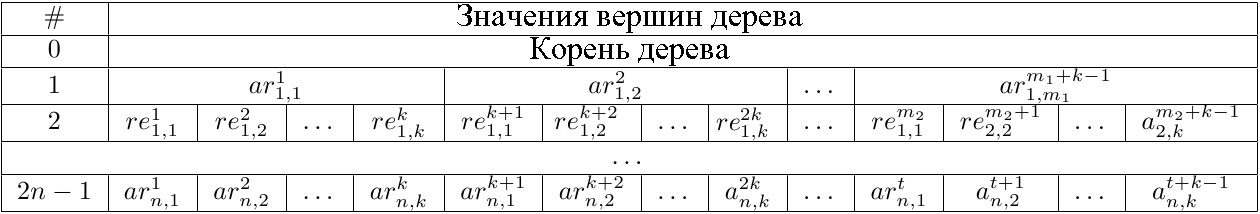
\includegraphics[width=\linewidth,keepaspectratio]{an_tbl2}
%\caption{Дерево изображений, универсум}
%\label{universum}
%\end{figure}

\section{Масштабные ряды}
Расширим базовую формализацию, добавив в качестве основного вполне упорядоченное множество $ScaleLine$, которое соответствует масштабному ряду (аналог масштабного ряда топографических карт 1:500,  1:1000 и т.д.), а также два дополнительных отношения: $Scale$,  которое связывает дуги с элементами $i$-являющейся образом $arc$ при сжатии изображения, т.е. при переходе к следующему (большему на единицу) элементу масштабного ряда.

При практической реализации удобно считать  вполне упорядоченное множество $ScaleLine$ отрезком натуральных чисел $[1,.., n]$ (это представление будет использоваться в статье для упрощения обозначений). В частности, поэтому будем использовать ниже конструкции вида: $s1  = s2 - 1$ и $s2  = s1 + 1$, где $s1$, $s2$  принадлежат  множеству $ScaleLine$.

Предполагаем,  что анализируемое изображение и образцы имеют представления для всех элементов масштабного ряда $ScaleLine$. Таким образом, совокупность всех дуг $A$ четырехосновной а.с.\ref{eq:model} может быть представлено в виде
\begin{equation}
A = A_1 \bigcup A_2 \bigcup ... \bigcup A_n
\label{eq:components_set}
\end{equation}
где  множества $A_i$ состоят из дуг, относящихся к $i$ - му элементу масштабного ряда. 

\begin{definition}
В дальнейшем множества дуг $A_i$ будем называть $i$-ой компонентой изображения.
\end{definition}


\begin{remark}
Для общего подхода, охватывающего все варианты сжатия изображения, включая рассмотрение  под углом (что, конечно,  не соответствует генерализации для топографических карт, где используется ортогональная проекция,  но весьма важно для практики, достаточно  вспомнить о зрении живых организмов, где обрабатываются зрительные образы правого и левого глаза), представление масштабного ряда $ScaleLine$ отрезком натуральных чисел $[1,.., n]$ или даже частично  упорядоченными множествами недостаточно. В дальнейшем для формализации масштабных рядов  будут использоваться многоосновные а.с., включающие частично упорядоченные множества и дополнительные множества с определенными на них отношениями. 
\end{remark}

Первое отношение
$$Scale: \varsigma \in A \times ScaleLine$$  %3
определяет принадлежность дуги отрезку масштабного ряда ScaleLine, т.е.
$$(Scale(a, s_1) \;\wedge\; Scale(a, s_2) \;\wedge\; s_1\leq s \leq s_2) \to Scale(a, s) $$

Как отмечалось выше,  отношение  $Scale$  обладает следующим основным свойством. Пусть 
$$A_i = \{arc_1, arc_2, ..., arc_r\}$$ %4
совокупность всех дуг $i$-го множества из объединения \ref{eq:components_set}. Тогда всегда  $Scale(arc_k, i)$  для всех $k$.  

Другим основным  свойством отношения  $Relation$ является следующее: $Relation$  может связывать только дуги, принадлежащие одному элементу масштабного ряда, т.е., если $Relation(rel, a_1, a_2)$, то существует элемент  $s$ из  $ScaleLine$ такой, что   $Scale(a_1, s)$,  $Scale(a_2,  s)$.

Второе отношение
$$Include: \varsigma \in A \times A$$  %5
определяет вложение дуги $a_1$   в дугу $a_2$   большего элемента масштабного ряда, т.е., если $Include ( a_1, a_2)$,  то  существует  $s$ из  $ScaleLine$ такой, что $Scale(a_2, s)$,  $Scale(a_1,  s)$  и   $Scale(a_1,  s-1)$.

Определим основные свойства отношения вложения  $Include$,  которые математически формулируются следующим образом:
\begin{enumerate}
\item $(Include ( a_1, a_2) \wedge  Include ( a_1, a_3) ) \to a_2 = a_3$; %6
\item $( s_1  = s_2 - 1 \wedge  Scale(a_1, s_1)) \to \exists a_2 : Scale(a_2, s_2) \wedge Include(a_1, a_2)$; %7
\item $(s_1  = s_2 - 1 \wedge Scale(a_1, s_2)) \to \exists a_2: Scale(a_2, s_1)\wedge Include(a_2, a_1)$; %8
\end{enumerate}
Переформулируем  основные свойства отношения вложения $Include$  более понятным образом, через отображения  $F_i$  определяемые отношением вложения  $Include$  из  множеств  $A_i$ в множества $A_i+1$ .     
Определим последовательность функций сжатия  $F_i : A_i \to A_{i+1}$ следующим образом: 
\begin{equation}
F_i(arc1) = arc2 \leftrightarrow Include ( arc_1, arc_2 )
\label{eq:include_prop1}
\end{equation}
где  дуга  $arc_1$  из множества $A_i$  , а  дуга  $arc_2$  из множества $A_{i+1}$.

\begin{lemma}
Функция сжатия  $Fi$ , заданная формулой \ref{eq:include_prop1},   всюду определена, однозначна (т.е. отображение)  и   является эпиморфизмом.
Доказательство следует из определения отношения $Include$,  и свойств 1,2,3 отношения $Include$.
\label{lemma:scale1}
\end{lemma}


\begin{remark}
В силу леммы \ref{lemma:scale1}  в дальнейшем во многих случаях вместо отношения $Include$  будем использовать совокупность отображений  $F_i$, которые будем называть сжатиями при переходе от  $i$-го  к $i+1$-ому  элементу масштабного ряда, где  $i \geq 1$ и  $i < n$.
\end{remark}

Следующее основное свойство определяет сохранение отношения связности $Relation$ дуг при сжатии, $$(F_i (arc_1) = arc_3\wedge F_i (arc_2) = arc_4 \wedge arc_3 \neq  arc_4   \wedge  Relation(rel, arc_1, arc_2)) \to Relation(rel, arc3_, arc_4)$$

\begin{definition}
Подмножество дуг $B = \{b_1, b_2, ..., b_s\}$  $i$  компоненты $A_i$ \ref{eq:components_set} назовем  связным, если для любых двух дуг $b_i$, $b_j$, существует последовательность дуг $c_1, c_2, ..., c_u$  из   $B$ такая, что  каждая пара дуг $c_v$, $c_{v+1}$ являются связанными,  $c_1 = b_i$ , $c_u = b_j$ .
\end{definition}

Прежде всего, необходимо доказать, что прообраз и образ связного множества остается связным, что и показывает следующая

\begin{lemma}
Пусть подмножество дуг $B = \{b_1, b_2, ..., b_s\}$  $i$-компоненты $A_i$ \ref{eq:components_set}  является связным, причем  $i > 1$.  Далее, пусть  $B_1$ ($B_2$) подмножества дуг $i-1$ компоненты $A_{i-1}$  (соответственно,  $i+1$ компоненты $A_{i+1}$), которые будем   называть прообразом  (соответственно,  образом)  подмножества  дуг $B$ относительно функций сжатия \ref{eq:include_prop1} , которые строго определим следующим образом: 
$$B_1 = \{b\; |\; b \in A_{i-1}, F_{i-1} (b) \in B \} $$
$$(\text{соответственно},\; B_2 = {b | b \in A_{i+1} , b  = F_i (b_j)  для некоторого b_j \in B })$$
Тогда подмножество дуг  $B1$ (соответственно,   $B2$) является связным.
\end{lemma}
\begin{proof}
Пусть  $d_1$, $d_2$   произвольные дуги из $B_1$  (соответственно, $B_2$ ). Тогда по определению $B_1$  (соответственно,   $B_2$ ) в подмножестве дуг $B$ существуют  дуги  $b_l$, $b_k$  такие, что $F_{i-1}(d_1) = b_l$, $F_{i-1} (d_2) = b_k$ (соответственно,  $F_i (b_l) = d_1$ , $F_i (b_k) = d_2$).

Так как  подмножество дуг $B$ является связным, то  существует последовательность дуг  $c_1, c_2, ..., c_u$  из   $B$ такая, что  каждая пара дуг $c_v,$ $c_{v+1}$ являются связанными,  $c_1 = b_l , c_u = b_k$. 

Определим  последовательность дуг $e_1, e_2, ..., e_u$ из $B_1$ (соответственно, $B_2$) следующим образом:
\begin{enumerate}
\item $e_1 = d_l$ , $e_u = d_2$, отметим, что $F_{i-1} (e_1) = c_1$ , $F_{i-1} (e_u) = c_u$ (соответственно,  $F_i (c_1) = e_1$, $F_i(b_k) = d_2$)
\item $F_{i-1}(e_j) = c_j$  (соответственно,  $F_i (c_j) = e_j$)   для всех $j$  из отрезка  
$[2, u - 1]$.
\end{enumerate}
Тогда  последовательность дуг $e_1, e_2, ..., e_u$ из $B_1$ (соответственно, $B_2$) такая, что  каждая пара дуг $e_v$, $t_{v+1}$ являются связанными по основному свойству отношения $Relation(rel, arc_1, arc_2)$, и  $e_1 = d_l$, $e_u = d_2$, что показывает связность подмножеств дуг $B_1$ (соответственно, $B_2$).
\end{proof}

Важным является следующее  
       
\textbf{Следствие.}
Прообраз  подмножества, состоящего из одной дуги, относительно функций сжатия  $F_i$ \ref{eq:include_prop1}, является связным.

\subsection{Результаты}
Теперь можем приступить  к доказательству основной цели работы: того, что, если сжатый образец изоморфно вложен в сжатое изображение (предполагается, что образцы и изображения используют один и тот же масштабный ряд), то исходный  образец может быть изоморфно вложен в исходное изображение, тогда и только тогда, когда прообраз каждой дуги образца может быть изоморфно вложен в прообраз соответствующей дуги изображения.

Во избежание громоздкого «всеобщего случая» будем рассматривать изоморфное вложение одного образца, представленного многоосновной  а.с.  
\begin{equation}
S  = < A_s, R_s, V_s, M_s; Sector, Angle, Relation >,                     %(9)
\label{scale:results:template}
\end{equation}
          
в изображение,  представленное многоосновной а.с.  
\begin{equation}
W  = < A_w, R_w, V_w, M_w; Sector,  Angle, Relation >                     %(10)
\label{scale:results:image}
\end{equation}

\begin{equation}
A_s = A_{s_1} \cup A_{s_2} \cup ... \cup A_{sn}  (A_w = A_{w_1} \cup A_{w_2} \cup ... \cup A_{w_n})                     %(11)
\label{scale:results:image}
\end{equation}
где  множества   $A_{s_j}$ (соответственно,  $A_{w_j}$) состоят из дуг, относящихся к $j$ - му элементу   масштабного ряда \ref{eq:model}. 
Будем считать, что последовательность функций вложения  
\begin{equation}
F_i : Ai \to A_{i+1}  %(12)
\label{scale:results:func1}
\end{equation}

определена на множествах дуг $A_s$  и $A_w$.  Тогда совокупность дуг $A_{s_2}$ (соответственно,  $A_{w_2}$) является  сжатием   совокупности дуг   $A_{s_1}$ (соответственно,  $A_{w_1}$)    и  $F_1 ( A_{s_1})  =  As2$ (соответственно,  $F_1 ( A_{w_1} )  =  A_{w_2}$) .  

\begin{definition}
Пусть $\varsigma : A_{s_2} \to A_{w_2}$  произвольное отображение. Отображение $\xi : A_{s_1} \to A_{w_1}$ назовем экстраполяцией отображения $\varsigma$ , если для любой дуги   $arc$  из $A_{s_1}$ выполняется:  пусть $\xi(arc)  =  arc_1$,   тогда  $\varsigma (F_1(arc) )  =  F_1(arc_1)$. 
\end{definition}
          
\begin{theorem}
Пусть  $\varsigma: A_{s_2} \to A_{w_2}$  изоморфное вложение сжатой совокупности дуг $A_{s_2}$ из $S$ \ref{eq:include_prop1} в  сжатую  совокупность дуг $A_{w_2}$ из  $W$ \ref{scale:results:image}. Тогда  изоморфное вложение   $\varsigma$  может быть экстраполировано  до  изоморфного вложения  $\xi: A_{s_1} \to A_{w_1}$ тогда и только тогда, если   для любой дуги $arc$ из $A_{s_2}$ прообраз  (относительно  функции сжатия  $F_1$)  дуги  $arc$ может быть изоморфно вложен в прообраз  (относительно  функции сжатия  $F_1$)   дуги $\varsigma(arc)$.                 
\end{theorem}            
\begin{proof}
Предположим, что  прообраз каждой дуги $F_{i-1}(arc)$ образца $A_{s_2}$  может быть изоморфно вложен в прообраз соответствующей дуги изображения  $F_{1-1}(\varsigma (arc))$  изображения  $A_{w_2}$.  Обозначим через  $\xi_{arc}$ такое изоморфное вложение, т.е.  $\xi_{arc} : F_{1 -1}(arc) \to F_{1 -1}(\varsigma (arc))$.  
Положим вложение $\xi = \xi_{arc_1} \cup \xi_{arc_2} \cup ... \cup \xi_{arc_L}$, где $A_{s_2} = \{arc_1, arc_2, ..., arc_L\}$. Тогда $\xi$ является изоморфным вложением, причем  экстраполированным  с изоморфным вложением  

$\varsigma : A_{s_2} \to A_{w_2}$ (следует из того, что $\xi_{arc} : F_{1 -1}(arc) \to F_{1 -1}(\varsigma (arc))$ ) и достаточность для теоремы  доказана.    
Докажем необходимость. Пусть $\varsigma : A_{s_1} \to A_{w_1}$ является изоморфным вложением из совокупности дуг образца  $A_{s_1}$  в совокупность дуг  изображения  $A_{w_1}$ экстраполированным  с изоморфным вложением  $\varsigma : A_{s_2} \to A_{w_2}$.  Тогда ограничение вложения  $\xi$  на  $F_{1 -1}(arc)$  будет изоморфным вложением в $F_{1 -1}(\varsigma (arc)$  для всех дуг  $arc$  из  совокупности  $A_{s_2}$. 
\end{proof}          

\begin{remark}
Конечно, программная реализация масштабных рядов и обеспечение эффективной работы функций сжатия $F_i$ \ref{scale:results:func1}  (а также обратных функций $F_{i -1}$)  требует  значительных усилий, которые должны быть «вознаграждены» повышением эффективности поиска изоморфных вложений образцов, что и будет показано во второй части данной работы.
\end{remark}

Пусть каждая из многоосновных а.с. R1 , R2 , …, Rm  вида (1)  имеет не  более   n   дуг и представляет связное изображение. Тогда анализ  связного изображения, представленного  многоосновной а.с.  D,  имеет верхнюю границу сложности не превышающую O(((w + t)*w) + m),  где  w (t) – количество дуг (соответственно, связей дуг) изображения, представленного  многоосновной а.с. D.  
           Пусть  многоосновные  а.с.  
              Sh  = < Ash, Rs, Vs, Ms; Sector,  Angle, Relation >,                      (13)
  
               (Wh  = < Awh, Rw, Vw, Mw; Sector,  Angle, Relation >)              (14)    
получены из многоосновной  а.с. S (9) (соответственно,  W (10) ) уменьшением множества дуг до  относящихся только к h - му элементу   масштабного ряда (11),  где  h  изменяется  от 1  до  n.  Положим также, что количество дуг в множестве  Awh равно  dh.                
	Для наших целей будет удобна  теорема  А в следующей формулировке.	Теорема Б.  Построение изоморфного  вложения  многоосновной  а.с. Sh  (13) в многоосновную  а.с. Wh  (14) имеет верхнюю границу сложности не превышающую O((dh + t)* dh),  где  dh (t) – количество дуг (соответственно, связей дуг) многоосновной  а.с. Wh  (14).
	Замечание 4. Возможность использования  одной и той же совокупности связей Rs  ( Rw ) для всей совокупности  многоосновных  а.с. Sh  (соответственно,  Wh) следует по основному свойству (*),  которое сохраняет  отношение связности Relation дуг при сжатии.  Хотя, конечно, при сжатии некоторые связи дуг могут становиться ненужными и учет этого, улучшил бы  оценку теоремы  Б.    
%	Определение 3.	Коэффициентом сжатия i –го  вложения  Fi : Ai → Ai+1                                                                   (12) будем называть отношение количества дуг множеств Ai и Ai+1   и будет обозначаться в дальнейшем Ei.    
%	Теорема 2.  Пусть  ζ : As2 → Aw2  изоморфное вложение сжатой совокупности дуг   As2  из S  (9) в  сжатую  совокупность дуг Aw2 из  W (10). 
%Тогда  построение изоморфного вложения  ξ : As1 → Aw1,   экстраполированого с  ζ, имеет верхнюю границу сложности не превышающую O((E1 + t)* d2),  где  d2 (t) – количество дуг (соответственно, связей дуг) многоосновной  а.с. W2  (14).            
%	Доказательство.  В силу Теоремы 1 необходимо проверить для любой дуги   arc  из As2  (дает коэффициент d2) изоморфное вложение  ее прообраза  в  прообразы дуги ζ (arc) (дает коэффициент  (E1 + t) ). Умножив данные коэффициенты,  получим оценку теоремы.                        
	Замечание 5.   1) Оценка сложности вычислена с большим запасом, т.к., например, в качестве коэффициента  d2  можно было взять количество  дуг именно   As2., а не количество  дуг  Aw2.
	2)  Совмещение деревьев интерпретаций   многоосновных  а.с. S1  и  S2 существенно улучшило бы оценки последней теоремы, но имеет большие технические трудности и не может быть представлена  в этой работе.
	Теорема 3.  Использование изоморфного вложения сжатого образца, представленного  многоосновной  а.с.  S2,  уменьшает сложность построения изоморфного вложения исходного образца, представленного  многоосновной  а.с.  
 S1.            
	Доказательство. Прямое применение оценок  Теоремы Б   дает верхнюю границу сложности изоморфного вложения исходного образца, представленного  многоосновной  а.с.  S1  не превышающую O((d1 + t)* d1) , где  d1 = d2 * E1 , а верхняя граница  сложности изоморфного вложения исходного образца, педставленного  многоосновной  а.с.   S1  с использование изоморфного вложения сжатого образца, представленного  многоосновной  а.с.  S2 дает оценку O((d2 + t)* d2) +  O((E1 + t)* d2) =  O((d2 + E1 + 2 * t ) * d2 ) заведомо меньшую, так как коэффициент сжатия на практике для более или менее сложных изображений всегда более 10.
	Теорема доказана.    
                        
4. Заключение. 
Программная реализация предложенного подхода будет иметь существннно большую эффективность, чем приведенные оценки  Теоремы 3. Это связано с тем, что использование изоморфного вложения сжатых образцов предполагает:
1) Совмещение деревьев интерпретаций для всего масштабного ряда образцов, что существенно облегчает проверку изоморфной вложимости пробразов дуг относительно функций сжатия  Fi. 
2) Исключение «лишних» дуг при сжатии, т.е. параметр t оценок эффективности  для сжатых образцов (а тем более для прообразов дуг) будет заведомо меньшим.  

%\section{Постановка задачи распознавания}
%Общую схему решения комбинаторных задач высокой сложности логико-эвристическими методами можно трактовать как отображение начальной (инициальной) многоосновной алгебраической системы.
%\begin{equation}
%\mathfrak{M_{ini}} = <A_1,...,A_s;f_1,...,f_n;p_1,...,p_k>
%\label{eq:init}
%%\label{eq:model}
%\end{equation}
%где $A_i$ -- основные множества, $f_i$ -- операции (функции) на основных множествах, $p_i$ -- предикаты (отношения) на основных множествах, в конечную (финальную) $\mathfrak{M_{fin}}$, удовлетворяющую ограничениям $\mathfrak{R_1,R_2,...,R_m}$.
%
%
%Уточним формализацию описания плоских контурных изображений для данного варианта проверки выполнимости ограничений.
%
%В качестве составляющих элементов образцов и анализируемого изображения выступают, очевидно, дуги и связи дуг.
%

%
%Соглашения по представлению элементов схемы~\ref{universum} следующие:
%
%\begin{enumerate}
%\item для элемента $\alpha_{\mu,\chi}^\theta$ - число $\theta$ является позицией на этаже схемы (номер клетки в строке); $\alpha_{\mu,\chi}^\theta$ является $\chi$-ым элементом из множества $Arc_{\mu}$ или $Rel_{\mu}$;
%\item числа $m_i$, где $i$ - номер этажа, равны $k^i - k$; число $t = k^{2n-1}-k$, отметим, что данные числа имеют чисто технический характер и уменьшают громоздкость выражений, стоящих в конце строк схемы~2.
%\end{enumerate}
%
%Очевидно, что схема~\ref{universum} содержит все изображения, имеющие не более $n$ дуг, и $k$ 
%вариантов дуг и связей дуг. 
%Структуру дерева на схеме~\ref{universum} будем задавать отношениями 
%$Par_{arc}(x,y)$, $Brot_{arc}(x,y)$ для дуг, и $Par_{rel}(x,y)$ для связей дуг.
%
%Отношение $Par_{arc}(x,y)$ задает отношение «родитель-потомок» на 
%декартовом произведении $Arc \times Rel$,
%например, $Par_{arc}(ar_{i,j}^2, re_{i,w}^{k(j-1)+w})$, где $1 \le w 
%\le k$. Отношение $Par_{arc}(x,y)$ связывает элементы, расположенные на 
%соседних этажах, и может быть определено строго математически, а именно, 
%$Par_{arc}(\alpha_{\mu,\chi}^\theta, \beta_{\zeta,\eta}^\gamma)$ тогда и только 
%тогда, когда 
%\begin{enumerate}
%\item $\mu=\zeta$ или $\mu + 1 =\zeta$
%\item $(\theta - 1)k \leq \zeta \leq (\theta - 1)k + k-1$
%\end{enumerate}
%Отношение $Brot_{arc}(x,y)$ задает отношение «быть братом» на 
%декартовом произведении $Arc \times Arc$.
%Отношение  $Brot_{arc}(x,y)$  связывает элементы, расположенные на одном этаже 
%и связанные с одним элементом верхнего этажа отношением «ро\-ди\-тель-потомок», 
%и может быть определено строго математически, а именно, 
%$Brot_{arc}(\alpha_{\mu,\chi}^\theta, \beta_{\zeta,\eta}^\gamma)$ тогда и 
%только тогда, когда
%\begin{enumerate}
%\item $\alpha=\beta$;
%\item $\mu=\zeta$;
%\item $\theta < \zeta$ и $\theta-\zeta<k$, а также $[\theta / k ]>0$, где 
%операция $[ ]$ остаток от деления.
%\end{enumerate}
%Отношение $Par_{rel}$ задается по аналогии, на декартовом 
%произведении $Rel \times Arc$.
%
%\begin{remark}
%на практике универсум \ref{universum} не строиться а строится только его часть, состоящая из дуг и связей дуг многоосновных а.с.  $\mathfrak{R_1,R_2 , ..., R_m}$.
%\end{remark}
%
%Докажем следующую лемму:
%
%\begin{lemma}
%Верхняя граница сложности построения интерпретации $\xi$ для связного изображения~\ref{eq:model} не превышает $O(w+t)$, где  $w$ -- количество дуг, $t$ -- связей дуг.
%\label{lm:main1}
%\end{lemma}
%\begin{proof}
%\textbf{Основание индукции.} Пусть $i = 1$ и $Sector(ar_1) = (j, j)$ и 
%$$Rrel_1 = \{ re_i\;|\;Relation(re_i, Ar_1 , Ar_2),\;Ar_1 = ar_1 \vee Ar_2 = ar_1 \}$$
%%\begin{eqnarray*}
%$$Arr_1 = \{ aar_i\;|\;Relation(re_i, Ar_1 , Ar_2),\;re_i \in Rrel_1,\nonumber
%(Ar_1 = ar_1 \wedge Ar_2 = aar_i) \vee (Ar_2 = ar_1 \wedge Ar_1 = aar_i) \}.$$
%%\end{eqnarray*}
%Тогда полагаем $\xi(ar_1) = ar_{1,j}^j$, $\xi(re_i) = re_{1,v}^{(j-1)*k+v}$, где $re_i \in Rrel_1$, $Angle(re_i) = Angle(re_{1,v}) = v$. 
%Если $aar_i \in Arr_1$, то $$\xi(aar_i)=ar_{2,e}^{(d-1)*k+e},$$ где $d$ – позиция элемента $\xi(re_i)$ (т.е. $d =(j-1)*k+v$, $Sector(aar_i) = (e, e)$.
%
%Отметим, что $Par_{arc}(\xi (ar_1), \xi (re_i))$, $Par_{rel}(\xi (re_i), \xi 
%(aar_i))$, а также для любых $aar_i$ и $aar_j$ из $Arr_1$ выполняется 
%$Brot_{arc}(\xi 
%(aar_i), \xi (aar_j))$.
%
%Интерпретация $\xi$ продолжается для множества дуг 
%$$Arc_1~=~Arc~\setminus~(\{ ar_1\} \bigcup Arr_1),
%$$ множества связей дуг $$Rel_1 = Rel \setminus Rrel_1.$$
%
%\textbf{Индукционный шаг.} Пусть после $i$-го шага получены непустые множества дуг $Arr_i = \{ ar_{i_1}, ar_{i_2}, ..., ar_{i_w} \} $, $Arc_i = Arc_{i-1} \setminus Arr_i$, множества связей дуг $Rrel_i , Rel_i = Rel_{i-1} \setminus Rrel_i$, причем по аналогии с основанием индукции, дуги из множества 
%$\xi(Arr_i)$ располагаются на $2 * i + 1$ этаже схемы~\ref{universum}, связи дуг из множества $\xi(Rrel_i)$ располагаются на $2 * i$ этаже схемы~\ref{universum}.
%
%По алгоритму основания индукции будем проводить построения для каждой дуги $ar_\alpha \in Arr_i$ такой, что $ar_\alpha$ не принадлежит объединению $\{ar_1 \} \bigcup Arr_1 \bigcup ... \bigcup Arr_{i-1}$.
%Пусть $Sector(ar_\alpha) = (j, j)$ и 
%$$Rrel_{i+1,\alpha} = \{ re_s\;|\;R(re_s, Ar_1 , Ar_2),\;re_s \in Rel_i,\;Ar_1 = ar_\alpha \vee Ar_2 = ar_\alpha \}$$
%\begin{equation*}
%\begin{split}
%\shoveleft Arr_{i+1,\alpha} = &\{aar_u\;|\;R(re_s, Ar_1 , Ar_2), \\
%&(Ar_1 = ar_\alpha \wedge Ar_2 = aar_u) \vee (Ar_2 = ar_\alpha \wedge Ar_1 = aar_u)\}
%\end{split}
%\end{equation*}
%Пусть $\xi(ar_\alpha) = ar_{i+1,j}^\beta$.
%Тогда $\xi(re_s) =re_{i+1,v}^{(\beta-1)*k+v}$, где $re_s \in Rrel_{i+1\alpha}$, 
%$$Angle(res) = Angle(re_{i+1, v}^{(\beta-1)*k+v}) = v.$$
%Если $aar_u \in Arr_{i+1,\alpha}$, то $\xi(aar_u) = ar_{2,e}^{(d-1)*k+e}$, где $d$ – позиция элемента~$\xi(re_s)$ (т.е. $d =(\beta-1)*k+v)$, $Sector(aar_u)~=~(e, e)$
%
%Отметим, что $Par_{arc}(\xi(ar_\alpha), \xi(re_s))$, 
%$Par_{rel}(\xi(re_s),\xi(aar_u))$, а также для любых $aar_i$ и $aar_j$ из 
%$Arr_{i+1\alpha}$ выполняется $Brot_{arc}(\xi(aar_i), \xi(aar_j))$.
%
%Полагаем множество дуг $Arr_{i+1}$ равным объединению всех $Arr_{i+1\alpha},$ где $ar_\alpha$ произвольная дуга из множества $Arr_i$ такая, что $ar_\alpha$ не принадлежит объединению 
%$\{ar_1\} \bigcup Arr_1 \bigcup ... \bigcup Arr_{i-1}$, также множество связей дуг $Rrel_{i+1}$ полагаем равным объединению всех $Rrel_{i+1\alpha}$, соответствующие произвольным дугам $ar_\alpha$ из множества $Arr_i$ (смотри, выше).
%
%Интерпретация  $\xi$ продолжается для множества дуг
%$$Arc_{i+1} = Arc_i~\setminus~Arr_i,$$
%и для множества  связей дуг
%$$Rel_{i+1}=Rel_i~\setminus~Rrel_{i+1}.$$
%
%
%Так как по условию интерпретируемое изображение~\ref{eq:model}  является  связным, то процесс интерпретации $\xi$ будет закончен не более, чем за $w$  шагов индукции, где $w$ -- количество дуг.
%
%Отметим, что соответствие при построении интерпретации $\xi$  для любой дуги или связи дуг изображения~\ref{eq:model}  производится за  один шаг, так как «связывание», соответствующего элемента схемы~2,  производится вычислением одной арифметической формулы. Таким образом, лемма доказана.
%
%\end{proof}
%
%\begin{theorem}
%Пусть каждая из многоосновных а.с. $\mathfrak{R_1, R_2, ..., R_m}$ имеет не  более $n$ дуг и представляет связное изображение. Тогда анализ  связного изображения \ref{eq:model} имеет верхнюю границу сложности не превышающую $O(\;(w + t)*w + m\;)$, где  $w$ -- количество дуг ($t$ -- количество связей дуг) изображения \ref{eq:model}.
%\end{theorem}
%\begin{proof}
%Построим интерпретации всех многоосновных\\а.с. $\mathfrak{R_1, R_2, ..., R_m}$  на универсуме  \ref{universum} для всех изображений, имеющих не более  $n$ дуг, и  $k$ вариантов дуг и связей дуг (сложность этой процедуры, конечно, не входит в оценку доказываемой теоремы).
%
%Далее, пометим все вершины универсума \ref{universum} номерами многоосновных а.с., чьи элементы соответствуют этим вершинам. Каждой многоосновной а.с. $\mathfrak{R_i}$ сопоставим пару чисел $(a_i, b_i)$, где  $a_i$ – количество помеченных вершин \ref{universum}, соответствующих дугам, $b_i$ – количество помеченных вершин \ref{universum}, соответствующих связям дуг (конечно, помеченных номером $i$).
%
%Построим совокупность интерпретаций $\xi_1, \xi_2, ..., \xi_w$  на универсуме \ref{universum} (с помеченными вершинами), которые отличаются выбором первой дуги для основания индукции. А именно, интерпретация $\xi_1$ начинается традиционно с дуги $ar_1$ ,  интерпретация $\xi_2$  начинается с дуги $ar_2$ ,  и так далее. Последняя интерпретация  $\xi_w$ начинается, соответственно, с дуги $ar_w$.
%
%Введем для каждой интерпретации  $\xi_i$     множество пар  
%\begin{equation}
%(a_{i_1} , b_{i_1} ), (a_{i_2} , b_{i_2} ), ..., (a_{i_m} , b_{i_m} )
%\label{vipeq6}
%\end{equation}
%
%где  $a_{i_j}(b_{i_j})$  - количество помеченных $j$ вершин схемы~2, соответствующих дугам (соответственно, связям дуг), полученных для интерпретации $\xi_i$. Если пара $(a_{i_j}  ,b_{i_j})$  равна паре  $(a_j, b_j)$, то, таким образом, найдено изоморфное вложение $j$-го изображения (образца)  в анализируемое изображение~\ref{eq:model}.
%
%В силу леммы~\ref{lm:main1}, построение каждого отображения $\xi_i$  требует не более  $w + t$ шагов и, таким образом, верхняя граница сложности  поиска всех изоморфных вложений не более  $O(((w + t)*w) + m)$, где «добавка» $O(m)$ возникает из-за необходимости сравнивать пары~\ref{vipeq6} с парами  $(a_j, b_j)$.
%\end{proof}


%\begin{definition}
%Определим множество точек разбиение подпути $P = v_1, \dots v_n$ по углу сгиба в окрестности $\epsilon\in Z^+$
%$$V_{spiral}^P = \left\{ \min_{|r(h, v)|}(v_i, v_i+1)\;|\;Sign(r(h,v_i)) \neq Sign(r(h,v_{i+1})) \wedge i=1,n-1 \right\}$$
%\end{definition}


%\end{alg}
%\chapter{Оформление различных элементов} \label{chapt1}
%
%\section{Форматирование текста} \label{sect1_1}
%
%Мы можем сделать \textbf{жирный текст} и \textit{курсив}.
%
%%\newpage
%%============================================================================================================================
%
%\section{Ссылки} \label{sect1_2}
%Сошлёмся на библиографию: \cite{bib1}, \cite{bib2}, \cite{bib3,bib4,bib5}.
%
%Сошлёмся на приложения: Приложение \ref{AppendixA}, Приложение \ref{AppendixB2}.
%
%Сошлёмся на формулу: формула (\ref{eq:equation1}).
%
%Сошлёмся на изображение: рисунок \ref{img:knuth}.
%
%%\newpage
%%============================================================================================================================
%
%\section{Формулы} \label{sect1_3}
%
%\subsection{Ненумерованные одиночные формулы} \label{subsect1_3_1}
%
%Вот так может выглядеть формула, которую необходимо вставить в строку по тексту: $x \approx \sin x$ при $x \to 0$.
%
%А вот так выглядит ненумерованая отдельностоящая формула c подстрочными и надстрочными индексами:
%$$
%(x_1+x_2)^2 = x_1^2 + 2 x_1 x_2 + x_2^2
%$$
%
%При использовании дробей формулы могут получаться очень высокие:
%$$
%  \frac{1}{\sqrt(2)+
%  \displaystyle\frac{1}{\sqrt{2}+
%  \displaystyle\frac{1}{\sqrt{2}+\cdots}}}
%$$
%
%В формулах можно использовать греческие буквы:
%$$
%\alpha\beta\gamma\delta\epsilon\varepsilon\zeta\eta\theta\vartheta\iota\kappa\lambda\\mu\nu\xi\pi\varpi\rho\varrho\sigma\varsigma\tau\upsilon\phi\varphi\chi\psi\omega\Gamma\Delta\Theta\Lambda\Xi\Pi\Sigma\Upsilon\Phi\Psi\Omega
%$$
%
%%\newpage
%%============================================================================================================================
%
%\subsection{Ненумерованные многострочные формулы} \label{subsect1_3_2}
%
%Вот так можно написать две формулы, не нумеруя их, чтобы знаки равно были строго друг под другом:
%\begin{eqnarray}
%  f_W & = & \min \left( 1, \max \left( 0, \frac{W_{soil} / W_{max}}{W_{crit}} \right)  \right), \nonumber \\
%  f_T & = & \min \left( 1, \max \left( 0, \frac{T_s / T_{melt}}{T_{crit}} \right)  \right), \nonumber
%\end{eqnarray}
%
%Можно использовать разные математические алфавиты:
%\begin{eqnarray}
%\mathcal{ABCDEFGHIJKLMNOPQRSTUVWXYZ} \nonumber \\
%\mathfrak{ABCDEFGHIJKLMNOPQRSTUVWXYZ} \nonumber \\
%\mathbb{ABCDEFGHIJKLMNOPQRSTUVWXYZ} \nonumber
%\end{eqnarray}
%
%Посмотрим на систему уравнений на примере аттрактора Лоренца:
%
%$$
%\left\{
%  \begin{array}{rl}
%    \dot x = & \sigma (y-x) \\
%    \dot y = & x (r - z) - y \\
%    \dot z = & xy - bz
%  \end{array}
%\right.
%$$
%
%А для вёрстки матриц удобно использовать многоточия:
%$$
%\left(
%  \begin{array}{ccc}
%  	a_{11} & \ldots & a_{1n} \\
%  	\vdots & \ddots & \vdots \\
%  	a_{n1} & \ldots & a_{nn} \\
%  \end{array}
%\right)
%$$
%
%
%%\newpage
%%============================================================================================================================
%\subsection{Нумерованные формулы} \label{subsect1_3_3}
%
%А вот так пишется нумерованая формула:
%\begin{equation}
%  \label{eq:equation1}
%  e = \lim_{n \to \infty} \left( 1+\frac{1}{n} \right) ^n
%\end{equation}
%
%Нумерованых формул может быть несколько:
%\begin{equation}
%  \label{eq:equation2}
%  \lim_{n \to \infty} \sum_{k=1}^n \frac{1}{k^2} = \frac{\pi^2}{6}
%\end{equation}
%
%В последствии на формулы (\ref{eq:equation1}) и (\ref{eq:equation2}) можно ссылаться.
%
%%\newpage
%%============================================================================================================================
%
%\clearpage